\section{Empirical study: daily-driver laptops}
\label{sec:empirical}

The taxonomy is only useful if the local, measurable subset is actually measured on the class of machine people use. We summarize a public harness\footnote{Companion repository: LLM-Inference. Isolated subprocesses, schema-versioned JSON, median of trials after one warmup.} that holds prompt length, generation length, and trial policy fixed, and varies one family at a time and then in combination.

\paragraph{Hardware.}
Mac M3 with \textbf{24\,GB} unified memory---the canonical daily-driver laptop in this study---and Mac M5 Max (workstation-class M-series). Same prompts, same token counts, same config labels.

\paragraph{Default shape.}
\(T_p=512\), \(T_g=128\), unless noted. Models are mlx-community checkpoints (Llama~3.1, Mistral, Qwen, Gemma, and related presets). Configurations: \texttt{fp16}, \texttt{w8}, \texttt{w4}, \texttt{w2}, with optional \texttt{+kv\_cache} (4-bit KV) and \texttt{+prefill} (\(\texttt{prefill\_step\_size}=2048\) vs.\ 512).

\subsection{Weight quantization dominates the floor}

On Mac M3, Llama~3.1~8B (Table~\ref{tab:bits}):

\begin{table}[t]
  \centering
  \small
  \caption{Llama~3.1~8B weight-bit sweep on Mac M3 (24\,GB), \(T_p=512\), \(T_g=128\).}
  \label{tab:bits}
  \begin{tabular}{@{}lcccc@{}}
    \toprule
    Config & Peak GB & TTFT (ms) & tok/s & vs fp16 \\
    \midrule
    fp16 & 16.33 & 2637 & 5.8 & \(1.0\times\) \\
    w8 & 8.96 & 2775 & 11.3 & \(1.9\times\) \\
    w4 & 5.06 & 2738 & 20.5 & \(3.5\times\) \\
    w2 & 3.11 & 2826 & 35.8 & \(6.2\times\) \\
    \bottomrule
  \end{tabular}
\end{table}

FP16 at 16.3\,GB on a 24\,GB machine is not a daily driver: the OS and a browser barely fit. 4-bit is the knee of the memory--speed Pareto (Figure~\ref{fig:pareto}): the laptop stays a laptop. 2-bit wins the leaderboard and is the first place quality complaints concentrate; we treat it as a last resort, not a silent default. Across 14 M3-feasible presets the same pattern holds: fewer bits raise tokens/s because decode is bandwidth-bound~\eqref{eq:roofline}.

\begin{figure}[t]
  \centering
  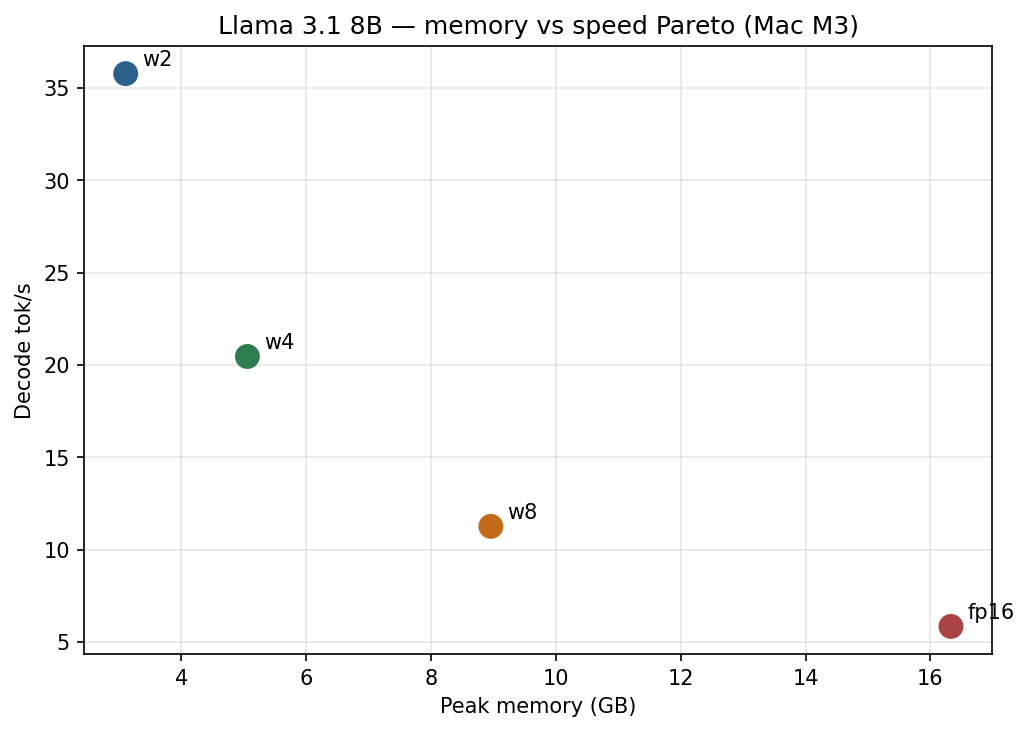
\includegraphics[width=0.98\linewidth]{figures/pareto.png}
  \caption{Memory--speed Pareto across weight bit-widths and models. Moving from FP16 to 4-bit is a joint win on both axes for bandwidth-bound decode---the difference between ``science fair'' and ``I leave this running all day.''}
  \label{fig:pareto}
\end{figure}

\subsection{Stacking KV quantization and prefill}

Table~\ref{tab:stack} is the capstone. Adding 4-bit KV and larger prefill chunks on top of 4-bit weights yields \textbf{5.06\,GB} and \textbf{19.9 tokens/s} for Llama~3.1~8B on M3 (\(\approx 3.55\times\) decode vs.\ FP16, \(\approx 31\%\) of FP16 memory). Mistral~7B moves from 3.6 to 16.0 tokens/s and 14.8 to 4.6\,GB (\(\approx 4.4\times\)). The \(\approx 11\)\,GB clawed back from Llama FP16 is enough to hold another 7--8B 4-bit model, or a fat RAG cache, \emph{or Chrome}.

\begin{table}[t]
  \centering
  \small
  \caption{Full stack on Mac M3 (24\,GB). Fully optimized \(=\) \texttt{w4+kv\_cache+prefill}.}
  \label{tab:stack}
  \begin{tabular}{@{}lccc@{}}
    \toprule
    Model / recipe & Peak GB & TTFT (ms) & tok/s \\
    \midrule
    Llama 3.1 8B, fp16 & 16.33 & 2689 & 5.6 \\
    Llama 3.1 8B, full stack & 5.06 & 2746 & 19.9 \\
    Mistral 7B, fp16 & 14.77 & 4350 & 3.6 \\
    Mistral 7B, full stack & 4.62 & 3954 & 16.0 \\
    \bottomrule
  \end{tabular}
\end{table}

TTFT barely moves on this \emph{short} prompt. That is expected: prefill's value shows up when \(T_p\) climbs. KV quantization's absolute gigabyte win is small at \(T=640\); it is insurance for long \(T\). On short chats, enabling KV+prefill on top of w4 can even cost a few tokens/s. Ship \texttt{w4+kv\_cache+prefill} as a \emph{product preset}; bench plain \texttt{w4} if you want peak short-chat speed.

At default \(T\), Llama~3.1~8B w4 vs.\ w4+KV on M3 is 20.7 vs.\ 20.4 tokens/s (about \(-1.5\%\)); Mistral and Qwen~2.5~7B similarly. The knob is not a dud---the benchmark is weight-dominated.

\subsection{The 16-config matrix on M5 Max}

Weight bits \(\times\) KV on/off \(\times\) prefill on/off is \(4\times 2\times 2 = 16\) configs. Table~\ref{tab:m5mat} (Llama~3.1~8B, M5 Max) shows the ladder: fp16 \(\approx 35\) tok/s at 16.5\,GB, w8 \(\approx 64\) at 9.0\,GB, w4 \(\approx 112\) at 5.1\,GB, w2 \(\approx 178\) at 3.3\,GB. KV and prefill barely change short-prompt decode. Mistral~7B on the same machine: fp16 \(\approx 37\) tok/s at 14.9\,GB \(\rightarrow\) optimized \(\approx 114\) tok/s at 4.7\,GB.

\begin{table}[t]
  \centering
  \small
  \caption{Selected cells of the Llama~3.1~8B matrix on Mac M5 Max (decode tok/s / peak GB).}
  \label{tab:m5mat}
  \begin{tabular}{@{}lcc@{}}
    \toprule
    Config & tok/s & Peak GB \\
    \midrule
    fp16 & 35.1 & 16.46 \\
    w8 & 63.6 & 8.97 \\
    w4 & 112.5 & 5.11 \\
    w4+kv+prefill & \(\approx 107\) & 5.11 \\
    w2 & 178.0 & 3.26 \\
    \bottomrule
  \end{tabular}
\end{table}

\begin{figure}[t]
  \centering
  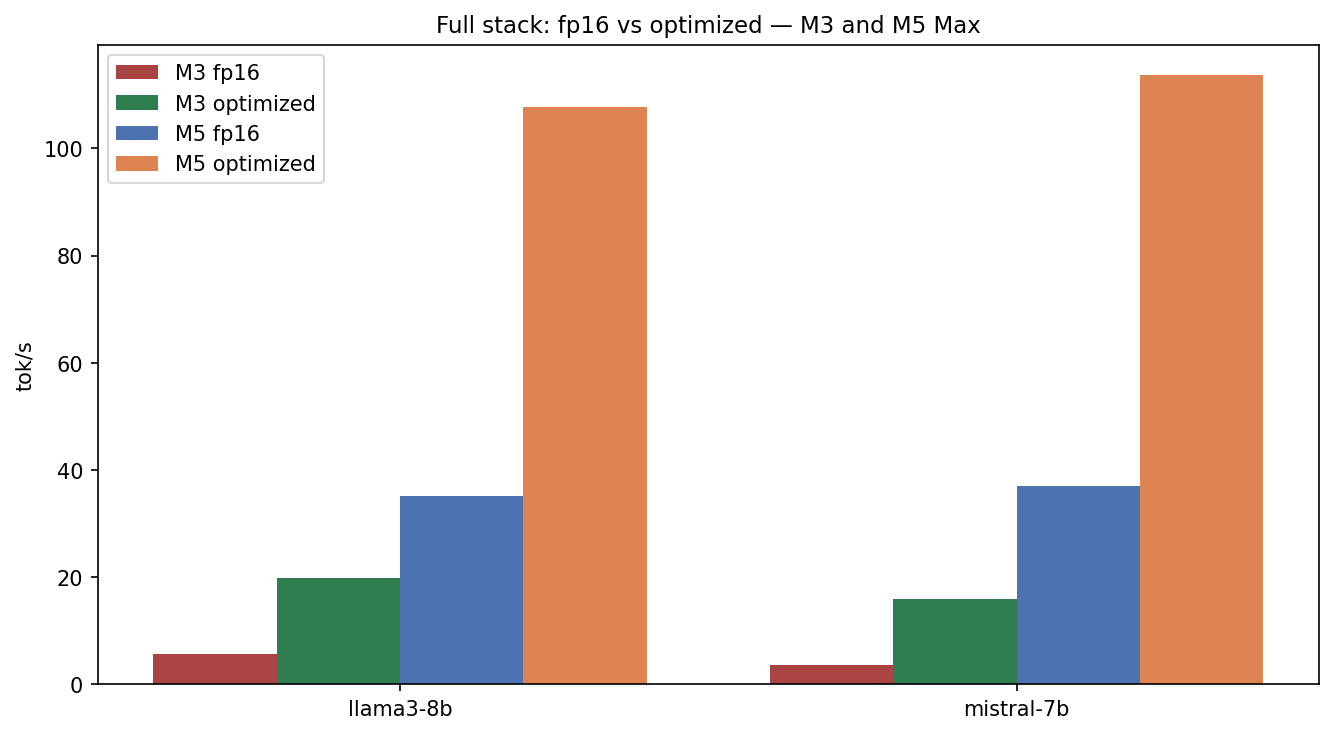
\includegraphics[width=0.98\linewidth]{figures/m3_m5_stack.png}
  \caption{Same software stack, two chips. Relative wins from leaving FP16 travel; absolute UX does not: \(\approx 20\) tok/s on M3 is usable chat, \(\approx 100+\) tok/s on M5 Max makes the UI the bottleneck.}
  \label{fig:m3m5}
\end{figure}

Relative stacking math is portable across M3 and M5. Absolute UX is not. Memory geometry is portable: \(\approx 5\)\,GB for an 8B w4 stack is the planning number on both. M5 makes ``FP16 for quality nights'' realistic (\(\approx 35\) tok/s); on M3, FP16 8B is a last resort.

\subsection{Model-size ladder}

Holding the recipe at 4-bit, M3 decode spans \textbf{238 tokens/s} at Qwen~2.5~0.5B (0.64\,GB) down to \textbf{20.6 tokens/s} at Llama~3.1~8B (5.06\,GB) and \textbf{15.4 tokens/s} at Gemma~2~9B (5.88\,GB)---about \(15\times\) from the tiny tier to the top of the ``real laptop'' tier before leaving single-digit billions of parameters (Figure~\ref{fig:ladder}). On M5 Max, Llama~8B 4-bit reaches \(\approx 112\) tokens/s and Gemma~27B 4-bit remains interactive at \(\approx 33\) tokens/s. Hardware bandwidth multiplies the same stack; it does not replace quantization on a 24\,GB machine. If you pick models by social-media vibes alone you will either swap a 70B to death or run a 0.5B and wonder why reasoning collapsed.

\begin{figure}[t]
  \centering
  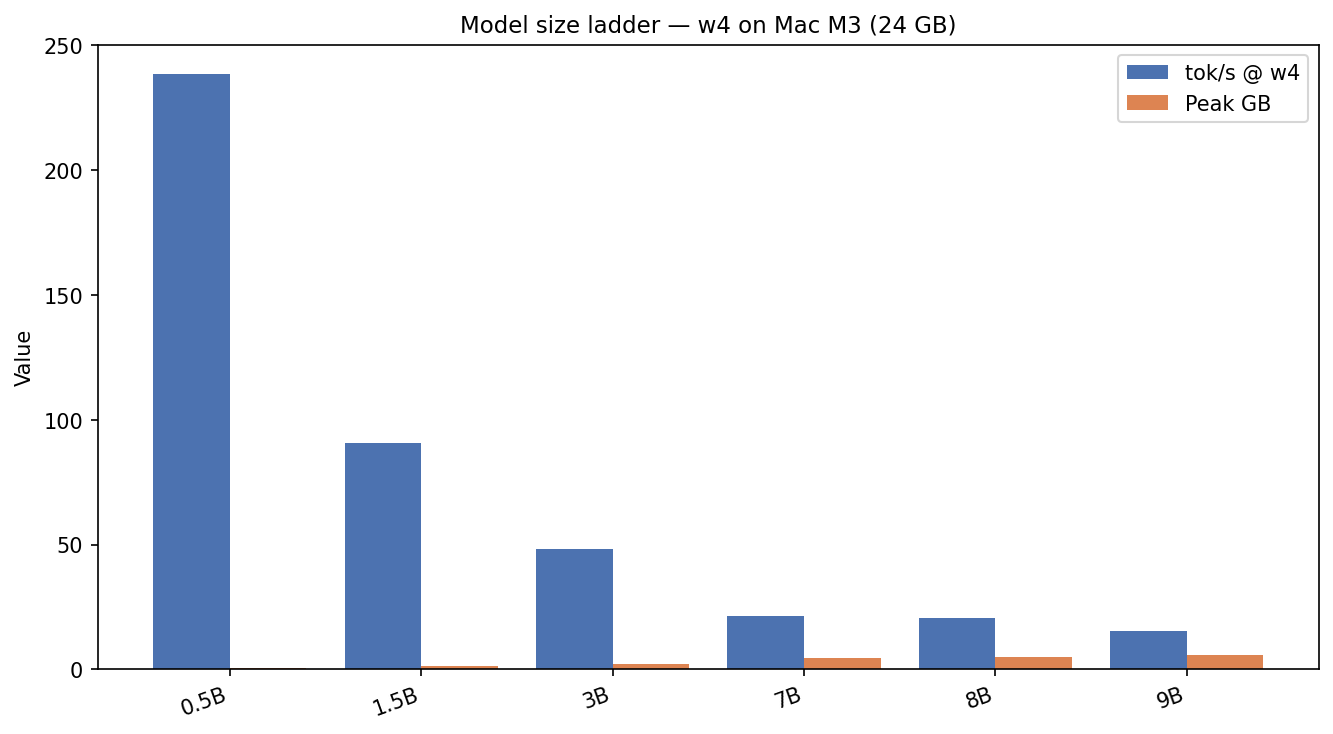
\includegraphics[width=0.98\linewidth]{figures/model_ladder.png}
  \caption{Dense 4-bit model ladder on Apple Silicon. Size is an inference optimization: quality, memory, and tokens/s move together.}
  \label{fig:ladder}
\end{figure}

\subsection{Speculative decoding is not unconditionally faster}

With a small 4-bit draft, Qwen~2.5~7B on M3 goes from 15.9 to \textbf{28.3 tokens/s} (\(1.78\times\)) at acceptance \(\alpha=74.2\%\), adding only \(\approx 0.3\)\,GB---possible only because 4-bit weights already freed RAM. The same pair on M5 Max goes from 122 to 170.3 tokens/s at the same \(\alpha\). Llama~3.1~8B on M5 Max is a negative result: 113.5 \(\rightarrow\) 109.7 tokens/s at \(\alpha=58.6\%\). Speculation should be reported with \(\alpha\) and a baseline, never as a guaranteed badge on a laptop preset.

\subsection{Context, RAG, and prefix cache}

Prefill TTFT grows steeply with \(T_p\) (Figure~\ref{fig:ttft}). On M3 with Llama~3.1~8B w4: \(T_p=256\) \(\rightarrow\) 2.4\,s TTFT; \(T_p=512\) \(\rightarrow\) \(\approx 3.1\)\,s; \(T_p=1024\) \(\rightarrow\) 5.8\,s; \(T_p=2048\) \(\rightarrow\) \(\approx 15.4\)\,s. A \texttt{rag\_agent} workload with \(T_p=4096\) records TTFT \(\approx 31.1\)\,s on M3 versus \(\approx 1.5\)\,s on M5 Max. That is a product failure on the smaller chip even when decode tokens/s look acceptable. Prefix KV cache converts a repeated system prompt from a prefill into a cache hit. Generation-length sweeps confirm Equation~\eqref{eq:kv}: decode tokens/s decay slowly as attention over the cache grows; peak memory tracks \(T\).

\begin{figure}[t]
  \centering
  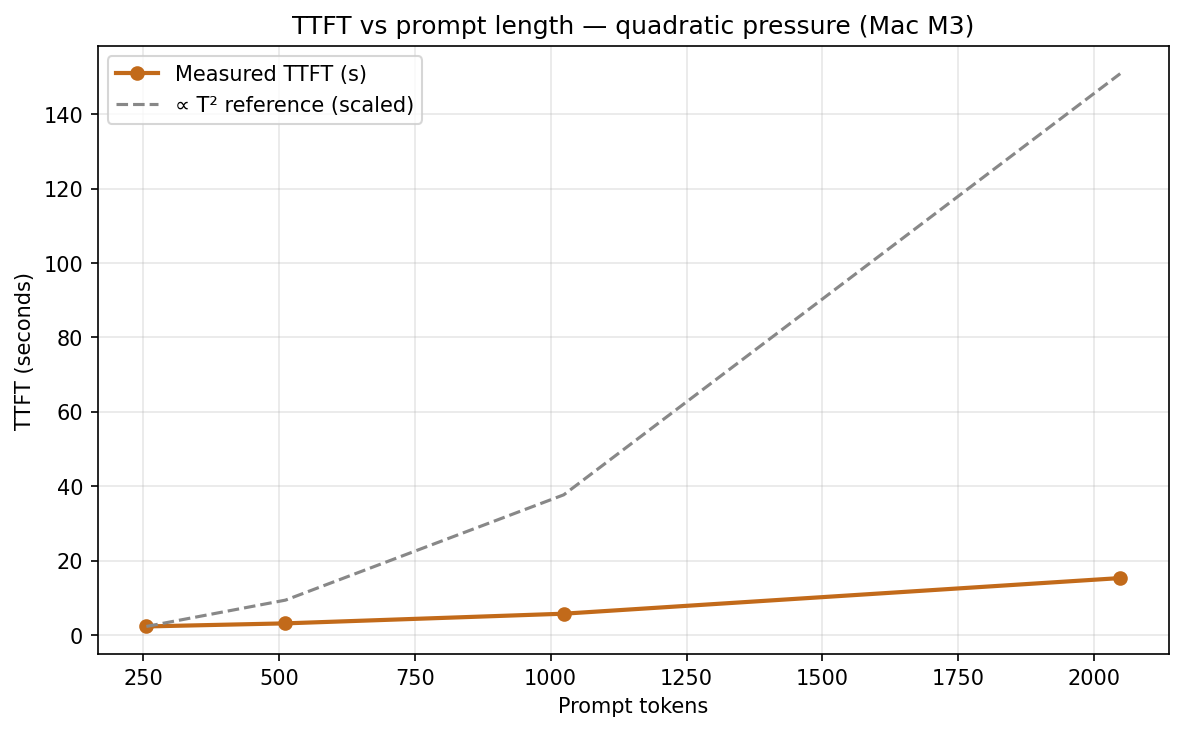
\includegraphics[width=0.98\linewidth]{figures/ttft_curve.png}
  \caption{TTFT versus prompt length. Local RAG dies in prefill, not in the tokens/s column. Everyday-device UX is a prefill SLO.}
  \label{fig:ttft}
\end{figure}

\subsection{Runtimes}

MLX and llama.cpp implement overlapping quant tiers on the same Metal GPU. In matched-tier comparisons (FP16 vs.\ F16 GGUF; 4-bit vs.\ Q4\_K\_M), neither engine universally wins; kernel quality, thread pinning, and quant layout dominate. Ollama is a packaging layer. The practical rule: pick the runtime that exposes the lever you need (MLX for Python sweeps; llama.cpp for portable GGUF and CPU fallback), then freeze it while you sweep \(b_w\) and \(T\).
